\documentclass{article}

% cool tables
\usepackage{booktabs}
\newcommand{\ra}[1]{\renewcommand{\arraystretch}{#1}}

\newcommand{\colorA}{\cellcolor{green!100}}
\newcommand{\colorB}{\cellcolor{green!60}}
\newcommand{\colorC}{\cellcolor{yellow!75}}
\newcommand{\colorD}{\cellcolor{orange!90}}
\newcommand{\colorE}{\cellcolor{red!80}}
% images
\usepackage{graphicx}
\usepackage{tabularx}
\usepackage{rotating}
\usepackage[table]{xcolor} 

% black square
\usepackage{amsmath}

\title{
    \normalsize \textsc{Rock Concert Audience as a Screen}\\
    \Huge Project plan}
\author{Agnethe Soraa,
Tomas Dohnalek,
Jan Bednarik,
Milos Jovac \\
\normalsize Project adviser: Anh Nguyen Duc}
\date{\today}

\begin{document}
\maketitle
\section{Project customer}
Netlight AS is a consulting company engaged in IT and management. They operates throughout Europe with offices in Stockholm, Oslo, London, Munich and Helsinki. The company was founded at 1999 and employs to 500 employees.

\section{Project description}
The customer wants a product to make the audience as a screen on a rock concert. We decided to name "digital lighter". 
The audience members at a rock concert should be able to download a simple application to their cell phone, and register this through a simple GUI.
Behind the artist on stage there is a screen, with a simple camera on top. The camera is taking pictures of the audience. 
At special occasions the audience will be instructed, by the artist, to hold up their phones with the screen towards the stage.
This is similar to holding up a lighter like people did in the old days to create a special atmosphere at the concert. 
We want to digitalize this by giving the audience a chance to use their cell phones instead of lighters. 

On control a signal the application will fill the entire mobile screen with a single colour.
The control signal can as an example say: "all pixels white". The signal will be specific for each application.
Each mobile will be a pixel in a larger picture, which will be presented on the big screen. 
What kind of picture the audience can create will depend on the number of people in the audience.   

As a motivation for the audience to hold up their phone, the camera on top of the screen will take pictures of the audience.
In that way the audience can see a reflection of them selves, and see what kind of picture they are creating together.  

\section{Required work}
- ?


\section{Project scope}


\section{Project architecture}
Product can be logically divided into two sections -- client and server application.
Client side should be used by the audience whereas server side should be used by the concert manager.
Both kind of applications will communicate through network, there is no need of internet connection.

Each application can be divided into more detailed architecture; we will focus on that in next sprint.


\section{Measurement of Project Effects}
To measure success of our end-product we have to set up some criteria to be fulfilled. The product should pass all test-cases and function according to customer's requirements.

\section{Planned workload}
Compendium proposed week workload 25 person-hours per week. During our internal meeting we have decided that each member will spend 30 hours per week because our team consists only of 4 members. We agreed on fixed daily working hours so that we could distribute the workload through the whole semester. We will do daily stand-ups according to Scrum methodology.

\section{General Terms}
\subsection{Methodology}
After fast research and consultation with our mentor, we decided to use SCRUM methodology for a 
few reasons. Requirements and scope of the undertaking were not that precisely defined at the time 
we had to decide on the methodology. Our approach therefore could not be founded on the sequential methodology as is "Waterfal".
We wanted to have frequent meetings with our customer and include him in development process. Sprints in SCRUM allow us just that - 
to have meeting with customer at the end of every sprint, and plan next one together. Sprints doesn't have to be the same length so 
we can better manage developing process and risks, and we will be able to have as much sprints as possible under time limit of 13 weeks. 
SCRUM will give us derivatives that we can enhance in increments and allow us to gradually reduce the risk and keep our customer informed 
about our progress. SCRUM is also a very popular approach in the software industry, so it is a good choice to learn it. 


\subsection{Tools selections}
For Scrum support and issue tracking we use Gravity Tool\footnote{www.gravitydev.com}. 
The tool is right now in Beta but it is free to use and have all features we needed from proposed AgileZen.
For collaboration on Minutes, Project Plan and other documents we use GitHub. This tool was proposed by out customer and it is popular free collaboration tool.
For document editing we agreed on LaTeX.
For group resources and links we use Facebook groups and for managing shedule we use Google Calendar.
 
\subsection{Limitations}
We should develop this project under a few technical, resource, time and knowlage limitations. 
Big limitation is image processing and small expirience in Mobile development.
As this course last for a 13 weeks, it is normal that we had to make some trade-offs. We devoted 2 weeks in exploring technologies and possible similar solutions that we can benefit from.
  
  
\section{Schedule}
general paragraph about sprint length
\subsection{Phases}
\paragraph{Sprint 0 (ends 6th of September)}
\paragraph{Sprint 1 (ends 20th of September)}
\paragraph{Sprint 2 (ends 4th of October)}
\paragraph{Sprint 3 (ends 18th of October)}
\paragraph{Sprint 4 (ends 1st of November)}
\paragraph{Sprint 5 (ends 15th of November)}
\subsection{Gantt chart}

\subsection{Milestones}

\begin{itemize}
    \item \textbf{Sprint 0}
    \item Project Plan
    \item Sprint 1
    \item Architecture design
    \item Simple GUI client \& server
    \item Sprint 2
    \item Implementation of client
    \item Set up protocol for client \& server
    \item Sprint 3
    \item Finish GUI client \& server
    \item Sprint 4
    \item Implementation of server
        \item Image processing
        \item Synchronization
    \item Sprint 5
    \item Evaluation
    \item Sprint 6
    \item Project Report
    \item Demo
    \item Presentation
\end{itemize}

\begin{figure}[ht]
\begin{center}
    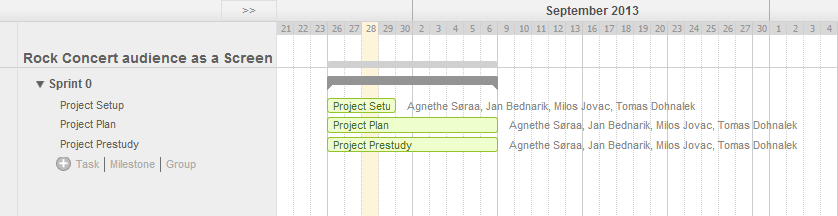
\includegraphics[scale=0.6]{images/gantt}
    \caption{Gantt Chart}
    \label{img:gantt}
\end{center}
\end{figure}
s
\section{Risk management}

\begin{table*}\centering \ra{1.3}
    \caption{Skills}
    \label{tab:skills}
    \vspace{2mm}
    \begin{tabular}{lcccc}
    \toprule
    \midrule
    \textbf{Event                	 } & Someone gets sick  		       & 1     & 2     & 3     \\ 
    \textbf{Consiquence              } & 4       					       & 1     & 1     & 1     \\ 
    \textbf{Possibility				 } & 5         						   & 1     & 4     & 1     \\ 
    \textbf{Risk                     } & 20        						   & 4     & 1     & 4     \\ 
    \textbf{Reactive Measures        } & Other people do more ours || Person can work from home         & 3     & 3     & 3     \\ 
    \textbf{Proactive Measures       } & Free weekends        			   & 3     & 1     & 2     \\ 
    \textbf{Responsible              } & All        					   & 2     & 5     & 1     \\ 
   
    \bottomrule
    \end{tabular}
\end{table*}

\begin{table*}\centering \ra{1.3}
    \caption{Skills and previous experience table. Coding:
        \textcolor{green!100}{$\bullet$} expert,
        \textcolor{green!60}{$\bullet$} experienced,
        \textcolor{yellow!75}{$\bullet$} neutral,
        \textcolor{orange!90}{$\bullet$} little experience,
        \textcolor{red!80}{$\bullet$} no experience}
    \label{tab:skills}
    \vspace{2mm}
    \begin{tabular}{lcccc}
    \toprule
                                & Agnethe   & Tomas & Milos & Jan \\
    \midrule
    \textbf{Leadership                 } & \colorB & \colorE & \colorD & \colorC \\ 
    \textbf{Scrum                      } & \colorB & \colorE & \colorE & \colorE \\ 
    \textbf{Mobile software development} & \colorC & \colorE & \colorB & \colorE \\ 
    \textbf{\LaTeX                     } & \colorE & \colorB & \colorE & \colorB \\ 
    \textbf{Network programming        } & \colorD & \colorC & \colorC & \colorC \\ 
    \textbf{Image processing           } & \colorE & \colorC & \colorE & \colorD \\ 
    \textbf{Java                       } & \colorC & \colorD & \colorA & \colorE \\ 
    \textbf{C++                        } & \colorE & \colorB & \colorC & \colorB \\ 
    \textbf{Testing                    } & \colorE & \colorB & \colorD & \colorC \\
    \bottomrule
    \end{tabular}
\end{table*}

\section{Organization}

\subsection{Role Assignment}
To assign roles according to our skills and previous experience we have decided to make survey of relevant knowledge. 
Results of this survey can be seen in table \ref{tab:skills}. 
This table was used as a base for our role assignment. 
The assigned roles can be seen in table \ref{tab:roles}. 
In the beginning we have decided to share other roles proposed by compendium.

\begin{table*}\centering \ra{1.3}
    \caption{Assigned roles and their responsibilities}
    \label{tab:roles}
    \vspace{2mm}
    \begin{tabularx}{\textwidth}{llX}
    \toprule
    Role    & Person   & Responsibility \\
    \midrule
    \textbf{Project Leader}             & Milos &
        Responsible for progress of the project according to the plan.
        Distributes work to group members.
        Has final call in arguments.\\
    \textbf{System Architect}             & Tomas &
        Check consistency and analyze all layers of the product. \\
    \textbf{Scrum Master}             & Agnethe &
        Leads the scrum stand-ups. \\
    \textbf{Communication Responsible}  & Jan &
        Responsible for communicating with customer and supervisor.
        Regularly send meeting minutes, agenda and other documents to customer and supervisor. \\ 
    \textbf{QA Responsible} & Tomas &
        Ensure a quality of all documents and end-product.
        \\ 
    \bottomrule
    \end{tabularx}
\end{table*}



\section{Risk management}

%\begin{sideways}
\begin{table*}\centering \ra{1.3}
    \caption{Handling risks}
    \label{tab:risks}
    \vspace{2mm} %\rotatebox{90}{
    \begin{tabularx}{\textwidth}{XlllXX}
    \toprule
        Event & Consequence & Possibility & Risk  & Reactive Measures & Proactive Measures \\
    \midrule
Someone gets sick & 4     & 5     & 20    & Other people do more work.  & Free weekends \\
Coding problems & 4     & 7     & 28    & Talk to supervisor \& Guru office & prepearing for the task \\
Testing problems & 4     & 4     & 16    & Talk to customer about reformulating requirements & Double check requirements with customer \\
Implementing things we are not supposed to & 7     & 6     & 42    & Try to adopt functionality or start all over & Don't do anything that is not in backlog and keep good communication with customer \\
Dead end with technologies & 8     & 8     & 64    & Talk to supervisor \& Guru office & Do thoroughly research \\
Unrealistic time estimate & 7     & 8     & 56    & Work overtime  & Planing poker \\
Frequent changes in requirements specification & 6     & 3     & 18    & Renegotiate with a customer & Try no to change finished modules and keep weekly meetings with the customer \\
Customer too ambitious & 9     & 5     & 45    & Renegotiate with a customer & Keep customer informed about what  to expect \\
Hardware problems & 9     & 3     & 27    & Obtain a new one & Keep your devices updated \\
    \bottomrule
    \end{tabularx}%}
\end{table*}
%\end{sideways}
\section{Quality Assurance}
Specific guidelines and practices were adopted
so that the team and the customer could continuosly verify that the project development keeps the right direction and that the requirements are being fulfilled.

\subsection{Customer collaboration}
Since the scope of the project and the actual requirements are determined by the customer it is essential to establish tight collaboration practises and even involve the customer in the collaboration tools the team uses. 

\paragraph{Meetings}
Considering this guidance we agreed on the weekly meetings. As the customer is located in Oslo the meetings will be carried out using the video-conference devices provided by the NTNU (accessible in the Accenture Lab) and Skype software. After each

\paragraph{Email}
Standard email messages will also serve the purpose of the communication mean, both team and thu customer agreed on responsing to the queries as soon as possible. 

\paragraph{Documents}
- minutes
- access to Drive
\paragraph{Other tools}
- Gravity, Skype conference, Google calendar







- meetings
- one person communicates
- customer decides about stories, accepts/rejects deliverable
- quality is determined by customer who ahs the opportunity to evalute the product (in its current state) after every sprint.


\subsection{Supervisor collaboration}
- one person communicates


\subsection{Team collaboration}
- continuous doc writing
- daily standups




\end{document}
